\chapter{Ejercicios}
\section{Tema 1}
\begin{ejer} [2] Demostrar que la condici\'on necesaria y suficiente para que tres puntos de un espacio proyectivo est\'en alineados es que los vectores que los representan sean linealmente dependientes.
\end{ejer}
\begin{sol}
    Sean $p_1, p_2, p_3 \in \mathbb P^n$, de forma que $p_i = \langle e_i\rangle$. 
    
    $\Rightarrow)$ $dim (p_1+p_2+p_3) = 2$ luego $p_1+p_2+p_3 = \mathbb P(E_3)$ para cierto $E_3$ con dimensi\'on 3, de forma que
    $$p_1+p_2+p_3=\pi(\langle e_1, e_2, e_3\rangle) = \pi(\langle e_1\rangle) + \pi(\langle e_2\rangle) + \pi(\langle e_2\rangle)$$
    y de esta forma, $\langle e_1, e_2, e_3\rangle = E_3 \iff \{ e_1, e_2, e_3\}$ son linealmente independientes.
\end{sol}

\begin{ejer}[9]
    Sea $\mathbb P^n$ un espacio proyectivo y $X$ e $Y$ dos subvariedades proyectivas de $\mathbb P^n$ que no se cortan. Demostrar que $X + Y = P$ si y s\'olo si $dim X + dim Y = dim \mathbb P^n - 1$.
\end{ejer}
\begin{sol}
    $\Rightarrow)$ $dim (X+Y) = dim X + dim Y - \cancelto{-1}{dim X\cap Y} = dim X + dim Y + 1 = dim \mathbb P^n$, luego $dim X + dim Y = dim \mathbb P^n - 1$

    $\Leftarrow)$ $dim X + dim Y = dim \mathbb P^n - 1$, entonces
    $$dim \mathbb P^n = dim(X+Y)=dim X + dim Y + 1 $$
\end{sol}
\begin{defi}
    Dadas dos subvariedades $X, Y \subset \mathbb P^n$, diremos que son \textbf{suplementarias}\index{Subvariedades suplementarias} si $X \cap Y = \emptyset$ y $X + Y = \mathbb P^n$.
\end{defi}
\begin{obs}
    Al hacer la radiaci\'on, usamos la variedad suplementaria al v\'ertice para proyectar.
\end{obs}
\begin{ejer}
    [13] Demostrar que dadas tres rectas cualesquiera $r_1, r_2, r_3$ de $\mathbb P^4$ que no est\'an contenidas en un mismo hiperplano y que son disjuntas dos a dos, existe una \'unica recta $\ell \subset \mathbb P^4$ que corta a las tres rectas $r_1, r_2, r_3$.
\end{ejer}
\begin{sol}
    Crearemos los hiperplanos que contiene a cada par de rectas. Sea $H_{12} = r_1 + r_2$, $H_{ij}$ de forma que $dim(H_{ij})=3$. As\'i, 
    $$H_{12} \cap H_{13} \cap H_{23} = \ell $$
    y por la propiedad de que no se cortan 2 a 2, $\ell$ es una recta, y es \'unica por construcci\'on. Aseguramos que $\ell$ y $r_1$ se cortan por ser $\ell, r_1 \subset H_{12} \cap H_{13}$, que es un plano, y dos rectas en el plano siempre se cortan.
\end{sol}

\section{Tema 2}
\begin{ejer}
    [1] Sea $\tau : \mathbb P^n \to \mathbb P^n$ una proyectividad inducida por la aplicaci\'on lineal $f : E \to E$. Probar que un punto $\langle e \rangle = p \in \mathbb P^n$ de $f$ es fijo por $\tau$ si y s\'olo si $e$ es un vector propio de $E$.
\end{ejer}
\begin{obs}
    La noci\'on de vector propio no depende del representante, ya que si $e$ lo es, 
    $$(\lambda f)(\mu e) = \lambda \mu f(e) = \lambda \alpha (\mu e)$$
\end{obs}
\begin{sol}
Por ser proyectividad, $\tau(p)=p \iff f(\langle e\rangle) = \langle e\rangle \iff f(e) \in \langle e\rangle \iff f(e)=\alpha e$. 
\end{sol}
\begin{ejer}
    [2] Construir una proyectividad $\tau : \mathbb P^n \to \mathbb P^n$  distinta de la identidad que deje fijos $n + 1$ puntos de $\mathbb P^n$ que sean proyectivamente independientes.
\end{ejer}
\begin{sol} Sean $\{p_0, \ldots, p_n\}$ los $n+1$ puntos.
    Elegimos representantes ($\langle e_i \rangle = p_i$), luego $\mathbb P(f) = \tau$. $f$ tiene, en la base $\{e_o, \ldots, e_n\}$ una base de vectores propios por el ejercicio anterior, luego diagonaliza y no es la identidad.

    De hecho, 
    $$\mathbb P(f) = Id \iff f=\lambda Id \iff \alpha_o = \cdots = \alpha_n$$

    Adem\'as, para que $\tau=Id$ es necersario que $\tau$ se la identidad en $n+2$ puntos, que formen sistema de referencia.
\end{sol}
\begin{ejer}
    [6] Sean $r$ y $s$ dos rectas de $\mathbb P^3$ que se cruzan, y 
    $\tau_r : r \to r$ y $\tau_s : s \to s$ dos proyectividades. Demostrar que existen infinitas proyectividades $\sigma : \mathbb P^3 \to \mathbb P^3$ tales que $\sigma|_r = \tau_r$ y $\sigma|_s = \tau_s$.
\end{ejer}
\begin{sol}
    En espacios vectoriales, $\mathbb P^3 = \mathbb P(E_4)$, $r=\mathbb P(F_2)$ y $s = \mathbb P(\bar{F_2})$. Adem\'as, tenemos que $\tau_r = \mathbb P(f_r)$ y $\tau_s = \mathbb P(f_s)$. 

    As\'i, se tiene que $E_4 = F_2 \oplus \bar{F}_2$ siendo $F_2 = \langle e_1,e_2 \rangle$ y $\bar F_2 = \langle \bar e _1, \bar e _2 \rangle$. En estas bases, asociaremos a las aplicaciones las matrices, $f \mapsto B_r$ y $f_s \mapsto B_s$.

    De esta forma, $g \mapsto B_{rs}$ para cierta $g$ con $\mathbb P(g) = \sigma$. Adem\'as, se verifica $\forall \lambda, \alpha_1, \alpha_2 \in k^*$ que $\mathbb P(\lambda g) = \sigma$. Podemos tambi\'en multiplicar cada $f_r$ y $f_s$ por escalares, siendo $\mathbb P(\alpha_1 f_r) = \tau_r$ y $\mathbb P(\alpha_2 f_s) = \tau_s$
\end{sol}
\begin{cor}
    Dadas estas dos rectas, y ya que $r+s = \mathbb P^3$, podr\'iamos pensar que dadas sus respectivas proyectividades, conocemos la proyectivizaci\'on en el espacio generado por ellas. Pero justamente el problema nos dice que son infinitas. 
\end{cor}
\begin{ejer}
    [7] Encontrar una proyectividad $ Id \neq \sigma: \mathbb P(\mathbb R^2 ) \to \mathbb P(\mathbb R^2 )$ tal que $\sigma^ 2 = Id$, pero no exista ninguna aplicaci\'on lineal $f : \mathbb R^2 \to \mathbb R^2$ que la induzca y cumpla que $f^2 = Id$.
\end{ejer}
\begin{sol}
    Tenemos que $\mathbb P(f) = \sigma$. Por la segunda condici\'on, tenemos que el anulador sea distinto de $x^2-1$. 

    Por otro lado, por ser $\sigma^2 = Id$ pero $f^2 \neq Id$, entonces $$f^2=\lambda Id (\lambda \neq 0,1)\iff c_f(x) = x^2 - \lambda $$
    y adem\'as el polinomio no es de grado 1 por no ser una homotecia.

    Eligiendo una base, la matriz de $f$ ser\'a
    $$f \longmapsto \begin{pmatrix}
        0 & \lambda \\ 1 & 0
    \end{pmatrix}$$
    y $f$ no es una homotecia, y $f^2 = - \lambda Id$, pero $\sigma^2 = \mathbb P(f^2) = \mathbb P^2( - \lambda Id)= Id $
\end{sol}
\begin{ejer}
    [8] Construir una proyectividad del espacio proyectivo real $\mathbb P^3_{\mathbb R}$ que no tenga puntos fijos.
\end{ejer}
\begin{sol}
    Endomorfismo con pol caract sin raices. Podemos elegir, partiendo del ejercicio anterior $(x+1)^2$
\end{sol}

Hoja 4
\begin{ejer}
    [11] En un plano proyectivo $\mathbb P^2$ se consideran los cuatro puntos $A = (1, 0, 0), B = (1, 1, 1), C = (0, 1, 1)$ y $D = (-2, 1, 1)$. Comprobar que est\'an alineados y calcular la raz\'on doble $(A, B; C, D)$. Hallar el punto $A_o \in \mathbb P^2$ tal que $(A_o , B; C, D) = -1$.
\end{ejer}
\begin{sol}
    Est\'an alineados ya que $B-A=C$ y $-3A+B=D$. Elegimos la base normalizada $\{-A, B\}$, por lo que $D$ tiene por coordenadas $D=(3:1)$. Por tanto, $(A,B;C,D)=3$. 

    Para la segunda parte, tenemos que 
    $$-1=(A',B;C,D)=(C,D;A',B) = (C,D;B,A') $$
    y en ese sistema de referenica $A'=(1:-1) = (-1:1)$. Cogemos un sistema de referencia en $A,B,C,D$ y hallamos sus coordenadas homog\'eneas. 

    Otra forma es fijar $\{A,B,C\}$ como sistema de referencia, de forma que buscamos $A'=(x_o:x_1)$ en dicho sistema, tal que $(A' , B; C, D) = -1$. Como $C=(1:1)$ y $D = (3:1)$ y usando la f\'ormula de los determinantes
    $$\dfrac{\begin{vmatrix}
        x_o & 1 \\ x_1 & 1
    \end{vmatrix}\begin{vmatrix}
        0 & 3 \\ 1 & 1
    \end{vmatrix}}{\begin{vmatrix}
        x_o & 3 \\ x_1 & 1
    \end{vmatrix}\begin{vmatrix}
        0 & 1 \\ 1 & 1
    \end{vmatrix}} = \dfrac{(x_o-x_1) (-3)}{(x_o-3x_1)(-1)} = -1 $$ 
    $$\iff 3x_o+3x_1=x_o-3x_1 \iff \begin{cases}
        3x_o+6x_1 = 0\\x_o+3x_1=0
    \end{cases} \iff \begin{cases}
        x_o = 3 \\ x_1 =-1
    \end{cases}$$
    as\'i pues, $A'=(-4,-1,-1) = (4:1:1)$.
\end{sol}
\begin{ejer}
    [13] Calcular, por dos m\'etodos distintos, la raz\'on doble $(a, b; c, d)$ de las cuatro rectas siguientes de $\mathbb P^2$:
$$a \equiv x_o - x_1 + 2x_2 = 0, b \equiv x_o + x_1 - x_2 = 0, c \equiv 2x_o - 4x_1 + 7x_2 = 0, d \equiv 5x_o + x_1 + x_2 = 0$$
\end{ejer}
\begin{sol}
    Para hablar de la ra\'zon doble de cuatro rectas estas deben ser concurrentes. Veamos el punto de corte de las dos primeras:
    $$\begin{cases}
        x_o - x_1 + 2x_2 = 0 \\ x_o + x_1 - x_2 = 0
    \end{cases} \Rightarrow \begin{cases}
        x_2 = -2x_o \\ -2x_o -x_o=-3x_o
    \end{cases} \Rightarrow (1:-3:-3)=V$$
    y ese punto pertenece a las otras rectas. Estas rectas se pueden ver como la radiaci\'on de v\'ertice $V$, de forma que $dim \, \modulo{\mathbb P^2}{V} = 1$. Cortando estas rectas con otra recta, tenemos que

    \textcolor{red}{dibujo}

    Identificando as\'i $\modulo{\mathbb P^2}{V} \longrightarrow r$. Eligiendo $r \equiv x_o = 0$, podemos hallar los puntos de corte que ser\'an $r\cap a = \{(0:2:-1)\}$, $r\cap b=\{(0:1:1)\}$, $r\cap c = \{(0:7:4)\}$, $r\cap d\ = \{(0,1,-1)\}$ y para calcular su raz\'on doble, elegimos un sistema de referencia en $r$. Podemos usar la f\'ormula de los determinantes porque elegimos las coordenadas $x_o,x_1$.

    Estas cuatro rectas, por antiisomorfismo de ret\'iculo de las subvariedades del dual, son cuatro puntos, $p_a=(1:-1:2), p_b=(1,1,-1), p_c = (2:-4:7), p_d = (5:1:1)$. Adem\'as, $V$ va a la recta $r_V \equiv z_o-3z_1-2z_2=0$ en la que est\'an los puntos.   
\end{sol}
\begin{ejer}
    [19] Sean $(A, B, C, P, Q)$ cinco puntos distintos de una recta proyectiva. Sabiendo que $(A, P; B, C) = (A, B; Q, C) = -1$ calcular $(A, Q; C, P)$.
\end{ejer}  
\begin{sol}
    $$(A, Q; C, P)=1-(A, C ; Q ,P) =1-(A,C;Q,B)(A,C;B,P) =$$ $$ =1- \left(\dfrac{1}{(A,C;B,Q)} \cdot \dfrac{1}{(A, P,B,C)}\right) = \cdots $$
\end{sol}
\begin{ejer}
    [14] Hallar, por dos m\'etodos distintos, la raz\'on doble $(H_1, H_2; H_3, H_4)$, de los siguientes hiperplanos del espacio proyectivo $\mathbb P^3$: 
    $$H_1 \equiv -x_1 + 3x_2 = 0, H_2 \equiv x_2 = 0, H_3 \equiv 5x_1 - x_2 = 0, H_4 \equiv 4x_1 - 3x_2 = 0$$
\end{ejer}
\begin{sol} \textcolor{red}{MAL}
    Para hallar la raz\'on doble de cuatro hiperplanos, estos deben cortarse en una recta $r$. Una recta en $\mathbb P^3$ es una subvariedad de $dim \, r=1$, por lo que tendr\'a 2 ecuaciones impl\'icitas. As\'i pues, cortaremos dos planos para hallar el eje de la radiaci\'on $dim \, \modulo{\mathbb P^3}{r} = \dim\, \left(\modulo{\mathbb P(E_4)}{\mathbb P(E_2)}\right) = dim \, \mathbb P \left(\modulo{E_4}{E_2} \right) = 1$ ya que $\modulo{\mathbb P^3}{r} \equiv \{x_o=0, x_3=0\} = r^*$, es decir, la podemos identificar con una recta que corte a todos los planos. Esta es $r \equiv (r^*)^0 = <(1,0,0,0),(0,0,0,1)>\equiv \{x_1=x_2=0\}$.
    
    Cortando todos los hiperplanos con la recta , de forma que $r \cap r' = \emptyset$ se cruzan. As\'i, podemos hallar los puntos de corte de cada hiperplano, \textcolor{red}{TERMINAR $H_1 \cap r' = \{-x_1 + 3x_2 = 0, x_1=0, x_2=0\} = \{(0:3:1:0\}$, $H_2 \cap r' = \{(0:1:0:0)\}$, $H_3 \cap r' = \{(0:1:5:0)\}$ y $H_4 \cap r' = \{(0:3:4:0)\}$. Para hallar su raz\'on doble, definimos como siempre un sistema de referencia, etc.}

    De manera dual, estos planos son puntos en $\mathbb P^3$, luego los puntos son $p_1=(0:-1:3:0)$, $p_2=(0:0:1:0)$, $p_3=(0:5:-1:0)$ y $p_4=(0:4:-3:0)$. La subvariedad en la que est\'an los puntos es el dual del v\'ertice de la radiaci\'on, y dado que $dim \, r = 1$, $codim \, r = 3 - 1 = 2$, es un plano, y dado que $r=\{x_3=0\}$, entonces $r^* \equiv \theta_0=0,\, \theta_3=0$.
\end{sol}
\begin{ejer}
    [16] Sean $r, r'$ dos rectas en $\mathbb P^3$ que se cruzan. Sean $\pi_1, \pi_2, \pi_3, \pi_4$ cuatro planos distintos que contienen a $r$. Teniendo en cuenta que una proyectividad conserva la raz\'on doble, demostrar la siguiente igualdad de razones dobles $$
(\pi_1, \pi_2; \pi_3, \pi_4) = (\pi_1\cap r', \pi_2\cap r'; \pi_3\cap r', \pi_4\cap r')$$
donde la primera se entiende como cuatro puntos de la radiaci\'on de planos de base $r$ y la segunda como cuatro puntos de $r'$.
\end{ejer}
\begin{sol}
    Como $r \in \pi_i \forall i =1,\ldots, 4$, los planos forman una radiaci\'on de eje $r$, es decir, $\modulo{\mathbb P^3}{r}$ de $dim \, =1$. Esta radiaci\'on, como en el ejercicio anterior se puede identificar con una recta, que ser\'a nuestra $r'$, que es una proyectividad $\tau=\mathbb P(f)$ tal que $f: E_2 \longrightarrow E_2'$ es isomorfismo, con $r=\mathbb P(E_2)$ y $r'=\mathbb P(E_2')$. Por el ejercicio anterior, la primera raz\'on doble es la raz\'on doble de los puntos duales a esos planos, que est\'an alineados por ser un haz de planos, y para la segunda raz\'on doble, la proyectividad es una $r'$ es la radiaci\'on, tal que $r'=(p+r)\cap r'$, de forma que si $p_i \in \pi_i$, entonces $(p_1,p_2;p_3,p_4)$ es la raz\'on doble de los planos. \textcolor{red}{XD}

    $E_2' \simeq \pi(E_2') = \modulo{E}{E_2}$, y proyectando tenemos el morfismo de identificaci\'on de la radiaci\'on con una subv. supl.
\end{sol}

\section{Tema 3}
\begin{ejer}
    [1] Sea $\varphi$ la proyectividad del plano proyectivo real $\mathbb P^2$ definida por $$\begin{cases}
         x_o' = x_1 + x_2 \\ x_1' = x_o + x_2 \\ x_2' = x_o + x_1 \end{cases}$$
Demostrar que $\varphi$ es una homolog\'ia no especial. Hallar su v\'ertice, su eje y su raz\'on.
\end{ejer}
\begin{sol}
    La matriz es 
    $$\varphi \leadsto \begin{pmatrix}
        0 & 1 & 1 \\ 1 & 0 & 1 \\ 1 & 1 & 0
    \end{pmatrix} \leadsto f$$
    Como queremos que exista un punto doble, este es un vector propio, y como queremos que sea una recta de puntos dobles, es un subespacio de dimensi\'on 2 de vectores propios. El polinomio caracter\'istico es
    $$c_f(x) = x^3 - 3x -2 = (x+1)^2(x-2)$$
    comprobemos que los subespacios tienen dimensi\'on que les toca
    $$f+1\leadsto \begin{pmatrix}
        1 & 1 & 1 \\ 1 & 1 & 1 \\ 1 & 1 & 1 
    \end{pmatrix}$$
    por lo que el n\'ucleo tiene dimensi\'on 2. Es decir, $f$ diagonaliza y $\varphi$ es homolog\'ia.

    Para calcular el v\'ertice, hacemos $ker(f+1) = <e_o-e_1, e_o-e_2>$ y el eje tendr\'a por ecuaciones $x_o+x_1+x_2$. 

    En la base de vectores propios, la matriz de $f$ es 
    $$f \leadsto \begin{pmatrix}
        2 \\ & -1 \\ & & -1
    \end{pmatrix}\leadsto \begin{pmatrix}
        -2 \\ & 1 \\ & & 1
    \end{pmatrix}$$
    luego el m\'odulo es -2.
\end{sol}
\begin{ejer}
    [2] Determinar una homolog\'ia del plano proyectivo real $\mathbb P^2$, sabiendo que su eje es la recta de
    ecuaci\'on $x_o + x_1 - 2x_2 = 0$, su v\'ertice es el punto $(1, 1, 0)$, y transforma el punto $(0, 1, -1)$
    en el punto $(1, 0, 1)$. Decidir si se trata de una homolog\'ia no especial, y en caso afirmativo determ\'inese su raz\'on.
\end{ejer}
\begin{sol}
    Podemos trabajar en las coordenadas $\{V,p_1,p_2;u=(0,1,-1)\}$ con $p_1, p_2 \in $ eje y hacer un cambio de base a ellos. La condici\'on del punto $u$ nos da el m\'odulo y luego cambiamos de base. Otra opci\'on es trabajar en el sistema de los puntos del enunciado. 
\end{sol}
\begin{ejer}
    [3] Determinar una homolog\'ia del plano proyectivo real $\mathbb P^2$, sabiendo que su eje es la recta de ecuaci\'on $x_o - 2x_1 + 2x_2 = 0$, su v\'ertice es el punto $(2, 0, -1)$, y transforma el punto $(1, 1, 1)$ en el punto $(3, 1, 0)$. Decidir si la homolog\'ia es especial.
\end{ejer}
\begin{sol}
    Trabajamos en las coordenadas $\{(2, 0, -1), p_1,p_2 ; (1, 1, 1)\}$ con $p, p' \in x_o - 2x_1 + 2x_2 = 0 \equiv \{(0,1,-1), (2,1,0)\}$, es decir, se verifica el sistema
    $$\begin{cases}
        (2, 0, -1) + (p_o,p_1,p_2)+(p_o',p_1',p_2') = (1,1,1) \\  p_o - 2p_1 + 2p_2 = 0 \\ p_o' - 2p_1' + 2p_2' = 0
    \end{cases} \Rightarrow$$
    hallemos la matriz
    $$\begin{pmatrix}
        a & b & c \\ d & e & f \\ g & h & i  
    \end{pmatrix}$$
    de forma que el eje qude invariante, es decir, que sobre 3 puntos sea la identidad, o sobre dos vectores del mismo valor propio, sea, $(0,1,1)$ y $(2,0,-1)$. Por tanto
    $$\begin{cases}
        a+b=\lambda & d+e=\lambda \\ g+h=0 & b+c=0 \\ e+f=\mu & h+i=\mu \\ 2a-c=2\mu & 2d-f=0 \\ 2g-i=-\mu & b-c=\xi \\ e-f=0 & h-i=\xi
    \end{cases}$$
\end{sol}
\begin{ejer}
    [7] Dada la homolog\'ia especial de $\mathbb P^2 (\mathbb C)$ de ecuaciones $$\begin{cases}
        x'=y \\ y'=-x+2y \\ z' = -2x+2y+z
    \end{cases}$$
    sabemos que tomando como hiperplano del infinito el eje, podemos interpretarla como una
    traslaci\'on. Determinar dicho espacio af\'in (complementario en $\mathbb P^2$ de un hiperplano), as\'i como las ecuaciones de dicha traslaci\'on. Demostrar que una homología no especial es armónica si y solo si es involutiva (c\'iclica de orden 2).
\end{ejer}
\begin{sol}
    Ya que $\tau(0,0,1)=(0,0,1)$, este es el v\'ertice. Si no, har\'iamos, hallar\'iamos $\tau(p)$ y $\tau(p)'$ para dos puntos cualesquiera y cortar\'iamos las rectas estables $(p+\tau(p))\cap (p'+\tau(p'))$. Para hallar el hiperplano (recta), hallaremos otro punto tal que $z=(p+p')\cap(\tau(p)+\tau(p'))$. Sean $p=(0,1,0)$ y $p'=(1,0,0)$, entonces $\tau(p)=(1,2,2)$ y $\tau(p')=(0,-1,-2)$, por lo que 
    $$z=((0,1,0) + \lambda (1,0,0)) \cap ((1,2,2) + \mu(0,-1,-2)) = (0,2,2)$$
    luego $z+v = (0,2,2)+\mu(0,0,1) \equiv x_o=0$. Es decir, $H=x_o=0$ y el espacio af\'in es $x_1=x_2=0$. 

    Dadas las ecuaciones en coordenadas homog\'eneas, en coordenadas afines $\theta_i=\dfrac{x_i}{x_o}$
    $$\begin{cases}
        \theta_1'=\dfrac{-x_o+2x_1}{x_1} = -\dfrac{1}{\theta_1}+2 \\  \theta_2'=\dfrac{-2x_o+2x_1+x_2}{x_2}=\dfrac{-2}{\theta_2} + \dfrac{2\theta_1}{\theta_2}+1
    \end{cases}$$

    Una homología no especial es armónica si y solo si es involutiva (c\'iclica de orden 2).
    \begin{dem}
        $\Rightarrow)$ Como $\sigma \leadsto \left( \begin{smallmatrix}
            -1 \\ & 1 \\ & & \ddots 
        \end{smallmatrix}\right)$, entonces $\sigma\circ \sigma = Id$. 

        $\Leftarrow)$ Como $\sigma \circ \sigma = Id \iff \sigma^{2} = Id \iff x^{2}=1$, $c_f(x) = x^{2}-1= (x+1)^n(x-1)^n = \left|\begin{smallmatrix}
            x-1 \\ & x+1
         \end{smallmatrix}\right|=|xId-A| = 0$, lo cual es solo cierto si 1 y -1 son valores propios, es decir, si $f$ tiene por matriz $f \leadsto \left( \begin{smallmatrix}
            -1 \\ & 1 
        \end{smallmatrix}\right)$. No s\'e hacer el caso general con $\sigma^{2n} = Id$
    \end{dem}
\end{sol}
\begin{ejer}
    [9] Dada la proyectividad de $\mathbb P^1(\mathbb R)$ de ecuaciones
    $$\begin{cases}
        x'=-y+3x \\ y'=x-y
    \end{cases}$$
    determinar (por el n\'umero de puntos dobles) si es el\'iptica (sin puntos dobles), parab\'olica (un \'unico punto doble) o hiperb\'olica (dos puntos dobles).
\end{ejer}  
\begin{sol}
    La matriz de la proyectividad es $f \leadsto (\begin{smallmatrix}
        3 & 1 \\ 1 & -1
    \end{smallmatrix})$, luego su polinomio caracter\'istico es
    $$c_f(x) = (x-3)(x+1)-1=x^2-2x-4=(x+2)^2$$
    luego $f$ tiene dos valores propios iguales $\lambda=2$, de forma que el subespacio generado es totalmente is\'otropo y la proyectividad es hiperb\'olica. 
\end{sol}
\begin{ejer}
    [10] Disc\'utase el car\'acter de la siguiente familia de homograf\'ias reales, seg\'un el valor de $\lambda$:
        $$\theta \theta' + (\lambda - 4)\theta + (\lambda + 4)\theta' + 9 = 0 $$
\end{ejer}
\begin{sol}
    Dado que la matriz de $\tau$ puede tener 0,1 o 2 vectores propios, esos determinan el car\'acter de la matriz. Dada la ecuaci\'on,
    $$\theta'=\dfrac{-(\lambda-4)\theta-9}{\theta+(\lambda+4)} \Rightarrow \tau \leadsto \begin{pmatrix}
        4-\lambda & -9 \\ 9 & \lambda+4
    \end{pmatrix}$$
    y para estudiar los valores propios pues hacemos el polinomio caracter\'istico y distinguimos los casos del discriminante, de la ra\'iz de la soluci\'on.
\end{sol}
\begin{ejer}
    [23] \textit{Eje transversal de una proyectividad entre rectas}. Sea $\sigma : r \to r'$ una proyectividad entre dos rectas de $\mathbb P^2$, entonces al variar $A, B \in r$ los puntos construidos por: $$(A+\sigma(B)) \cap (B+\sigma(A))$$ yacen en una recta. Dicha recta se denomina eje transversal. Probar adem\'as que el eje transversal pasa por el punto $r \cap r'$ si y solo si $\sigma$ es una perspectividad. Enunciar los duales de las propiedades anteriores. Concluir que si $\sigma$ es una proyectividad entre dos haces de rectas tal que la recta que une los puntos base es invariante, entonces el conjunto de puntos $\{r \cap \sigma(r)\}$ al variar $r$ en el primer haz de rectas, define una recta.
\end{ejer}
\begin{sol}
    Supongamos que $\sigma$ no es perspectivdad, luego $\sigma(0)\neq 0$. En ese caso
    \textcolor{red}{DIBUJO}
    donde la recta $e\equiv u+v$ es el eje transversal. Hacemos pues
    $$\bt r \arrow{r}{\tau_{A'}} & e \arrow{r}{\tau_{A}} & r' \\[-5mm]
    0 \arrow[mapsto]{r} & v \arrow[mapsto]{r} & v\\[-5mm]
    u \arrow[mapsto]{r} & u \arrow[mapsto]{r} & 0\\ [-5mm]
    A \arrow[mapsto]{r} & A'' \arrow[mapsto]{r} & A' \et$$
    donde $\tau_A$ es unir con $A$ y cortar con el espacio de llegada. Por lo que $\sigma = \tau_{A} \circ \tau_{A'}$, es decir, toda proyectivdad entre subvariedades es producto de proyectividades. Para otro $B$, $\sigma(B) = \tau_A(\tau_{A'}(B))$
    $$\bt r \arrow{r}{\tau_{A'}} & e \arrow{r}{\tau_{A}} & r' \\[-5mm]
    B \arrow[mapsto]{r} & B''=(A'+B)\cap e \arrow[mapsto]{r} & (B''+A)\cap r' = \sigma(B)\et$$
    Aplicamos en estas condiciones el enunciado, por lo que cogemos las rectas que se consideran, de forma que por construcci\'on, se cortan en $e$. 
\end{sol}
\section{Ejercicios}
\begin{ejer}
    [9] Se consideran en el plano proyectivo $\mathbb P^2$ los cuatro puntos $p_o = (1 : 0 : 1), p_1 = (0 : 2 : 1), p_2 = (0 : 0 : 1), p_3 = (1 : -1 : 0)$. 
    \begin{enumerate}[a)]
        \item Comprobar que $\mathcal R = \{p_o, p_1, p_2; p_3\}$ es una referencia proyectiva, y buscar una base asociada a ella. 
        \begin{sol}
            Los vectores asociados a los puntos son $e_o=(1,0,1), e_1=(0,2,1), e_2=(0,0,1)$, y para que los puntos no est\'en alineados, basta que los vectores son linealmente independientes. En efecto, hacemos su determinante y es 2, por lo que son base. As\'i pues, tenemos que $\lambda_o e_o + \lambda_1 e_1 + \lambda_2 e_2 = (1,-1,0)$, y si todas las $\lambda_i \neq 0$, no est\'a en ninguna cara y por tanto ser\'ia sistema. En efecto
            $$(\lambda_o, 2\lambda_1, \lambda_o+\lambda_1+\lambda_2) = (1,-1,0) \iff \begin{cases}
                \lambda_o = 1 \\ 2\lambda_1=-1 \Rightarrow \lambda_1= -\nicefrac{1}{2} \\ \lambda_o+\lambda_1+\lambda_2 = 0 \Rightarrow 1- \nicefrac{1}{2} + \lambda_2=0 \Rightarrow \lambda_2=-\nicefrac{1}{2}
            \end{cases}$$

            La base normalizada asociada es simplemente $e_i'=\lambda_i e_i \, i =\{0,1,2\}$, de forma que ahora $e_o'+e_1'+e_2'=(1,-1,0)$, que era el punto unidad. Para que desaparezcan las fracciones elegimos $\bar{e}_i=2 e_i'$. Esta base tambi\'en es normalizada, pues $\bar{e}_o+\bar{e}_1+\bar{e}_2=(2,-2,0)$, que es tambi\'en un representante de $p_3$, luego $\{\bar{e}_o,\bar{e}_1,\bar{e}_2\}$ es una base normalizada.
        \end{sol}
        \item Calcular las coordenadas homog\'eneas respecto a $R$ del punto (1 : -2 : 1).
        \begin{sol}
        Basta hallar los escalares para los cual se verifica
            $$(1,-2,1) = \mu_o \bar{e}_o+\mu_1\bar{e}_1+\mu_2\bar{e}_2$$
        \end{sol}
        \item  Calcular las coordenadas homog\'eneas respecto a $\mathcal R$ de un punto arbitrario $(x_o : x_1 : x_2)$.
        \begin{sol}
            Para encontrar la expresi\'on de las nuevas basta invertir la matriz de cambio de base.
        \end{sol}
    \end{enumerate}
\end{ejer}
\begin{ejer}
    [10] Comprobar que los tres puntos $(1 : 2 : 2),(3 : 1 : 4),(2 : -1 : 2)$ de $\mathbb P^2$ est\'an alineados, y determinar una ecuaci\'on de la recta que pasa por ellos.
\end{ejer}
\begin{sol}
    Basta ver que los vectores asociados, $(1,2,2), (3,1,4),(2,-1,2)$, ya que generar\'ian un espacio de dimensi\'on 2, que proyectivizada ser\'ia una recta, estando alineados los puntos. 

    Vamos a expresar el subespacio vectorial como ecuaci\'on (luego proyectamos). Este subespacio es
    $$<(1,2,2),(2,-1,2)> \iff \begin{cases}
        x_o = \lambda +2\mu \\ x_1 = 2 \lambda- \mu \\ x_2 = 2\lambda + 2\mu 
    \end{cases}$$
    que en verdad son las coordenadas hom\'ogeneas, $(x_o:x_1:x_2)$. Para calcular la ecuaci\'on impl\'icita, calculamos el incidente al subespacio, es decir,  hacemos el determinante
    $$\begin{vmatrix}
        x_o & x_1 & x_2 \\ 1 &2&2\\2&-1&2
    \end{vmatrix} = 0 \iff 4x_o + 4x_1 -x_2 -4x_2-2x_1+2x_o=0$$
\end{sol}
\begin{ejer}
    [15] En el espacio proyectivo $\mathbb P^3$ hallar:
    \begin{enumerate}[a)]
        \item La ecuaci\'on del plano que contiene a la recta $r \equiv x_o - x_1 + x_2 = 0 = x_1 - 2x_2 + x_3$ y
        al punto $p = (1 : 2 : 0 : 1)$.
        \begin{sol}
            Lo primero de todo, $p \nin r$.
            
            La radiaci\'on de centro $r$ es un haz de planos con ecuaciones:
            $$\lambda(x_o-x_1+x_2) + \mu(x_o-2x_1+x_2)=0$$
            de forma que verifique que pase por $p$. Es decir, 
            $$\lambda(1-2)+\mu(2+1) = \iff -\lambda+3\mu =0 \iff \lambda=3\mu$$
            luego un caso es
            $$3 (x_o-x_1+x_2) + (x_o-2x_1+x_2)=0 \iff 4x_o-5x_1+4x_2=0$$
        \end{sol}
        \item  La ecuaci\'on del plano que pasa por los puntos (1 : 0 : 1 : 1), (1 : 0 : 3 : 2) y
        (5 : 2 : 0 : 1).
        \item Las ecuaciones de la recta que se obtiene al cortar el plano del apartado (b) con el
        plano que pasa por los puntos (1 : 1 : 1 : 2), (1 : 0 : 0 : 1) y (0 : 0 : 1 : 0).
    \end{enumerate}
\end{ejer}
Hoja 3
\begin{ejer}
    [2] Dados los sistemas de referencia en $\mathbb P^1$ $\mathcal R = \{ (5: 0), (1: -1), (2: -1)\}$, y $\mathcal R' = \{ (1: -1), (3: -1), (-2: 0)\}$. Dar una proyectividad que transforma el primero en el segundo.
\end{ejer}
\begin{sol}
    Si $\tau = \mathbb P(f)$, dicha $f: \mathbb R^2 \to \mathbb R^2$ verifica que
    $$\begin{cases}
        f(5,0) = \lambda_1(1,-1) \\ f(1,-1) = \lambda_2(3,-1)
    \end{cases}$$
    de forma que 
    $$\begin{pmatrix}
        a &b\\c&d
    \end{pmatrix}\begin{pmatrix}
        5\\0
    \end{pmatrix}=\begin{pmatrix}
        5a\\5c
    \end{pmatrix} = \lambda_1\begin{pmatrix}
        1\\-1
    \end{pmatrix}$$
    y 
    $$\begin{pmatrix}
        a-b\\c-d
    \end{pmatrix}=\lambda_2 \begin{pmatrix}
        3\\-1
    \end{pmatrix}$$
    y para el punto unidad
    $$\begin{pmatrix}
        2a-b\\2c-d
    \end{pmatrix}=\lambda_3 \begin{pmatrix}
        -2 \\ 0
    \end{pmatrix}$$
    teni\'endose el sistema
    $$\begin{cases}
        5a = \lambda_1 \\ 5c=-\lambda_1 \\ a-b=3\lambda_2 \\ c-d=-\lambda_2 \\ 2a-b=-2\lambda_3 \\ 2c-d=0
    \end{cases}$$
    las cuentas al que se quiera suicidar. Saldr\'a en funci\'on de un par\'ametro, el que acompaña a $f$.

    Otra forma de hacerlo es elegir una de las $\lambda_i = 1$, dividiendo el resto por ella. Es posible porque siempre ser\'a distinta de 0.
\end{sol}
\begin{ejer}
    [4] En el plano proyectivo $\mathbb P^2$ tenemos dos cuaternas de rectas $\{r_i\}_{i=1,...,4}$ y $\{r'_
i\}_{i=1,...,4}$ tales que ninguna de ellas contiene tres rectas concurrentes. Probar que existe exactamente una proyectividad $\varphi : \mathbb P^2 \to \mathbb P^2$ cumpliendo $\varphi(r_i) = r'_i$ para todo $i \in \{1, 2, 3, 4\}$.
\end{ejer}
\begin{sol}
    Es el dual del ejercicio anterior. Basta definir $\tau$ del ejercicio anterior por $\tau: (\mathbb P^2)^* \longrightarrow (\mathbb P^2)^*$ tal que $\tau(r_i^0) = (r_i')^0$. 
\end{sol}
\begin{ejer}
    [9] Hallar las ecuaciones de la proyectividad $\varphi \neq Id$ del plano proyectivo $\mathbb P^2(\mathbb R)$ que tiene por puntos fijos a (1, 0, 0), todos los de la recta $x_o = 0$, y adem\'as cumple $\varphi^2 (p) = p$ para todo punto $p$ de la recta $x_2 = 0$.
\end{ejer}\begin{sol} Sea la base normalizada $\{e_o,e_1,e_2\}$, la recta $x_o=0 \equiv \mathbb P(<e_1,e_2>)$. Tenemos $f: \mathbb R^3 \longrightarrow \mathbb R^3$ tal que $f(e_o)=\lambda_o e_o$, pero de la misma forma $e_1, e_2$. Es decir, todos son vectores propios, pero $e_1$ y $e_2$ tienen el mismo $\lambda$ por lo que la matriz de $f$ es 
$$f\leadsto \begin{pmatrix}
    \lambda_o \\ & \lambda \\ & & \lambda
\end{pmatrix}$$
Incluyamos ahora la \'ultima condici\'on. $f^2$ es 
$$f^2 \leadsto \begin{pmatrix}
    \lambda_o^2 \\ & \lambda^2 \\ & & \lambda^2
\end{pmatrix}$$
entonces $\lambda_o^2=\lambda^2$, de forma que $\lambda_o=\pm \lambda$. En el caso positivo, $f$ ser\'ia una homotecia por lo que $\varphi$ ser\'ia la identidad. As\'i pues solo queda que 
$$f \leadsto \begin{pmatrix}
    -1 \\ & 1 \\ & & 1
\end{pmatrix}$$
o cualquier m\'ultiplo suyo.
\end{sol}
\begin{ejer}
    [10] Estudiar si la aplicaci\'on proyectiva $\varphi: \mathbb P^3 \to \mathbb P^3$ de ecuaciones $x_o'=x_o, x_1'=x_3, x_2'=x_2, x_3'=x_3$ es una proyecci\'on. Calcular las im\'agenes y las im\'agenes inversas del punto $p = (1, -1, 0, -1)$ y de la recta $r \equiv x_1 = 0 = x_o + x_2 + x_3$.
\end{ejer}
\begin{sol}
    La matriz de la aplicaci\'on es
    $$f \leadsto \begin{pmatrix}
        1 & 0 & 0 & 0 \\ 0 & 0 & 0 & 1 \\ 0 & 0 & 1 & 0 \\ 0 & 0 & 0 & 1
    \end{pmatrix}$$
    de forma que $ker\, f = <e_1>$, y adem\'as $\mathbb P(f): \mathbb P^3 - \mathbb P(ker\, f) \longrightarrow \mathbb P^3$. 

    \textcolor{red}{FALTA}
    De forma que $Im \, f = <e_o,e_2,e_1+e_3>$ que es suplementario de $<e_1>$. 

    Por el paso al cociente anterior, $e_o \longmapsto e_o$, $e_2 \longmapsto e_2$ y $e_3 \longmapsto (e_3+<e_1> \cap Im f) = e_3+e_1$. esta proyecci\'on coincide con la dada, por lo que es una proyecci\'on.
    \textcolor{red}{TERMINAR}

    Sea la proyecci\'on $\pi : \mathbb P - V = \{(0:1:0:0)\} \longrightarrow \mathbb P(<e_o,e_2,e_1+e_3>)$.
    
    El punto verifica que $p \in \mathbb P(<e_o,e_2,e_1+e_3>)$. As\'i, $\pi^{-1}(p)=p+V=(0:1:0:0)+(1:-1:0:-1)$. De forma que las ecuaciones de la recta son $x_2=0, x_o+x_3=0$. 

    La recta $r \equiv x_1 = 0 = x_o + x_2 + x_3$. Los vectores directores de la recta son ciertos y se comprueba si son combinaciones lineales de $e_o, e_2, e_1+e_3$ para ver si est\'a en $W=\mathbb P(<e_o,e_2,e_1+e_3>)$. Si $r \subset W$, $\pi^{-1}(r) = r+V$. En otro caso, $r \nsubset W$, entonces $\pi(r)=(r+V)\cap W$
\end{sol}
\begin{ejer}
    [7] En el plano proyectivo real $\mathbb P^2$ se consideran los puntos $A = (1, -1, 0), B = (0, 1, -1)$ y $C = (1, 1, -2)$. Hallar otros dos puntos $C'$ y $D$ tales que $(A, B; C, D) = -\nicefrac{1}{2}$ y $(A, B; C' , D) = -\nicefrac{2}{3}$. 
\end{ejer}\begin{sol}
    Vemos si los puntos est\'an alineados. Entonces su determinante ser\'a 0. Veamos que en la recta $A+B=r$ con sistema de referencia $\{A,B;C\}$ tenemos que encontrar $C'$ y $D$. La base normalizada es 
    $$\lambda(1,-1,0)+\mu(0,1,-1)=(1,1,-2) \Rightarrow \begin{cases}
        \lambda=1 \\ -\lambda+\mu=1 \\ \mu=2
    \end{cases}$$
    y la base normalizada es $\{e_A=(1,-1,0),e_B=2(0,1,-1);e_C=(1,1,-2)\}$. De esta forma, $D$ en el sistema de coordenadas es $D=(-1:2)$, luego $D=<-e_A+2e_B=(1,-1,0)+4(0,1,-1) = (-1,5,4)>$.

    En el segundo caso, es equivalente a $(A, B; D, C') = -\nicefrac{3}{2}$, y se resuelve igual que el anterior. Ahora el sistema de referencia es $\{-e_A, 2e_B; e_D\}$, luego $-3e_A'+2e_B'=$
    
\end{sol}


 \section{Tema 4}
 \begin{ejer}
     En $\mathbb P^3$, se considera la cu\'adrica $C\equiv x_1^2+x_2^2 + x_3^2+x_4^2+2x_1x_2+2x_1x_3 + 2x_1x_4+2x_2x_3+2x_2x_4-2x_3x_4 = 0$. Calcular los hiperplanos $A_1x_1+\cdots +A_4x_4=0$ que son tangentes a $C$.
 \end{ejer}
 \begin{sol}
     Buscamos pues que $(A_1,A_2,A_3, A_4) \in (\mathbb P^3)^*$, est\'e en $\overline{C}^*$
     $$C \leadsto \begin{pmatrix}
         1 & 1 & 1 & 1\\ 1 & 1 & 1 & 1\\  1 & 1 & 1 & -1\\  1 & 1 & -1 & 1\\ 
     \end{pmatrix}= G$$
     que vemos claramente que es singular. Escogemos pues un menor distinto de $0$, $\Delta_{33}$, de forma que $\rad T_2 = <e_1-e_2>$, y fijamos un suplementario suyo $F=<e_2,e_3,e_4>$. De esta forma, eligiendo $\{\omega_i\}$ la base dual de $\{e_i\}$, $(\rad T_2)^0 = <\omega_1+\omega_2,\omega_3,\omega_4>$, y para que los hiperplanos sean tangentes a $C$, son hiperplanos que contienen a $V$, $A_1 = A_2$. 

     As\'i, $\overline{T}=T_2|_F \leadsto \left(\begin{smallmatrix}
         1 & 1 & 1  \\ 1 & 1 & -1  \\ 1 & -1 & 1  \\
     \end{smallmatrix}\right)=\overline G$ y entonces $\overline{T}_2^*$ tiene por matriz $\overline{G}^{-1} \leadsto\nicefrac{1}{2}\left( \begin{smallmatrix}
         0 & 1 & 1 \\ 1 & 0 & -1 \\ 1 & -1 & 0
     \end{smallmatrix}\right)$, y entonces si $F^*=< \overline{\omega}_2, \overline{\omega}_3, \overline{\omega}_4>$, por la matriz, 
     $$\overline{A}_2\overline{A}_3+\overline{A}_2\overline{A}_4-\overline{A}_3\overline{A}_4 = 0$$
     y falta ver la relaci\'on con $(A_1,A_2,A_3,A_4)$, de forma que fij\'andonos en $(\rad T_2)^0$, lo que ocurre es que $(\overline{A}_2, \overline{A}_3, \overline{A}_4) = (A_2,A_3,A_4)$, pues ya vimos que $A_1=A_2$. As\'i, los hiperplanos tangentes a $C$ son aquellos tal que 
     $$ A_1=A_2 \quad \wedge \quad A_2A_3+A_2A_4-A_3A_4 = 0$$
     \textcolor{red}{HAY QUE TENER MUCHO CUIDADO CON LAS COORDENADAS!! COMPROBAR QUE ES EL PLANO TANGENTE CON LAS DERIVADAS PARCIALES}
 \end{sol}
\begin{ejer}
    [8] Demu\'estrese que por cinco puntos distintos del plano proyectivo $\mathbb P^2$, cuatro de los cuales forman un sistema de referencia (o cuadriv\'ertice), pasa una \'unica c\'onica. Adem\'as la c\'onica es no degenerada (no singular) si el quinto punto no est\'a alineado con dos cualesquiera de los cuatro que forman la referencia.
\end{ejer}
\begin{sol}
    Sean $\{p_1,\ldots, p_5\}$ los puntos. Llamemos a la matriz $T_2 \leadsto \left( \begin{smallmatrix}
        a & b & c \\ b & d & e \\ c& e & f
    \end{smallmatrix}\right)$ tal que alguno de los 6 par\'ametros es no nulo. As\'i pues depende de 5 condiciones, es decir, 5 puntos, para que sea un sistema determinado. 

    \textcolor{red}{DIBUJO}
    Geom\'etricamente, entendemos que existe un haz de c\'onicas $<T_2,T_2'>$ dado por las c\'onicas formadas por las rectas que unen los puntos $p_1, \ldots, p_4$. A estos puntos, añadiendo los puntos diagonales del cuadrivértice, son los denominados \textbf{puntos fundamentales del haz de cónicas}.
\end{sol}
\begin{ejer}[9]
    Calcular las cónicas que pasan por $p_1=(0,1,1), \, p_2=(1,0,1), \, p_3=(1,1,0), \, p_4=(1,1,1), \, p_5=(0,2,1)$
\end{ejer}
\begin{sol}
    Se tiene que $\{p_1,p_2,p_3;p_4\}$ forman sistema de referencia, cuya base asociada es normalizada. As\'i, $p_5=3e_1-e_2+e_3=(0,4,2)=(0,2,1)$. Es decir, $p_5=(3,-1,1)$ en este sistema de referencia. 

    Escribiendo la matriz de la m\'etrica buscada en este sistema,
    $$T_2 \leadsto \begin{pmatrix}
        0 & a & b \\ a & 0 & c \\ b & c & 0
    \end{pmatrix}=G \Rightarrow 0 = (1,1,1)G \begin{pmatrix}
        1\\1\\1
    \end{pmatrix}=(a+b,a+c,b+c)\begin{pmatrix}
        1\\1\\1
    \end{pmatrix}=2a+2b+2c=0$$
    $$(3,-1,1) G \begin{pmatrix}
        3 \\ -1 \\ 1
    \end{pmatrix} = (-a+b, 3a+c,3b-c)\begin{pmatrix}
        3 \\ -1 \\ 1
    \end{pmatrix}=-6a+6b-2c=0$$
    luego 
    $$\begin{cases}
        a+b+c=0 \\ -3a+3b-c=0
    \end{cases}\Rightarrow \begin{cases}
        c=3a-3b \\ c=-a-b
    \end{cases} \Rightarrow \begin{cases}
        c=-3a \\ 2a=b
    \end{cases}$$
    luego 
    $$G=\begin{pmatrix}
        0 & 1 & 2\\ 1 & 0 & -3 \\ 2 & -3 & 0
    \end{pmatrix}$$
    luego la c\'onica es 
    $$-xy+2xz-3yz=0$$
    en el sistema de referencia $B=\{p_1,p_2, p_3;p_4\}$. Ahora falta hacer el cambio de base, cuya matriz ser\'a 
    $$B=\begin{pmatrix}
         0 & 1 & 1 \\ 1 & 0 & 1 \\ 1 & 1 & 0
    \end{pmatrix}$$
    y 
    $$G'=(B^{-1})^t G B^{-1}$$
\end{sol}
\begin{ejer}
    [11] Sea $\{p_1, p_2, p_3; u\}$ un sistema de referencia del plano proyectivo $\mathbb P^2$. Pru\'ebese que existe una \'unica c\'onica no degenerada que pasa por $p_1, p_2, p_3$ y cuyas tangentes en $p_1$ y $p_2$ son las rectas $T_{p_1}C\equiv p_1 + u$ y $T_{p_2}C\equiv p_2 + u$. 
\end{ejer}
\begin{sol}
    No puede ser degenerada, pues si lo fuera, $(p_1+u)(p_2+u)\equiv C$. Como $\{p_1, p_2,,p_3\}$ son is\'otropos
    $$T_2\leadsto \begin{pmatrix}
        0 & a & b\\ a & 0 & c \\ b & c & 0  
    \end{pmatrix}=G \equiv axy+bxz+cyz=0$$
    y añadimos las condiciones de tangencia, que nos dicen que la polar de cada $p_i=p_i+u$, que es la imagen de la polaridad asociada. As\'i, nos dice que $y-z=0, \, x-z=0$ (determinate si hace falta), luego 
    $$\phi_{T_2} \begin{pmatrix}
        1 \\ 0 \\ 0
    \end{pmatrix}=\begin{pmatrix}
        0 \\ 1 \\ -1
    \end{pmatrix}, \, \phi_{T_2} \begin{pmatrix}
        0 \\ 1 \\ 0
    \end{pmatrix}=\begin{pmatrix}
        1 \\ 0 \\ -1
    \end{pmatrix}\Rightarrow a=1, \, b=-1, \, c=-1$$
    Otra opci\'on es obligar a que 
    $$\begin{cases}
        y-z=0 \\ axy+bxz+cyz=0
    \end{cases}$$
    tenga una \'unica soluci\'on para que sea tangente, y ser\'a $p_1$. As\'i, 
    $$\begin{cases}
        y-z=0 \\ axy+bxz+cyz=0
    \end{cases} \iff \begin{cases}
        y=z \\ axy+bxz+cy^2=0 \Rightarrow 
    \end{cases}$$
    $$\Rightarrow y\big((a+b)x+c\big)=0 \Rightarrow (a+b)x+cy=0 \Rightarrow a+b=0 \Rightarrow b=-a$$
\end{sol}
\begin{ejer}
    [15] Dada la c\'onica $K \equiv x^2 + 2y^2 + z^2 + yz + 3xz + xy = 0$, y el punto $A = (1, 1, 1)$, se pide hallar:
    \begin{enumerate}
        \item Las tangentes a $K$ desde $A$.
        \item La polar de $A$ respecto de $K$. 
        \item Los puntos de intersecci\'on de la polar de $A$.
        \item El cono formado por las rectas tangentes a $K$ que pasan por $A$.
    \end{enumerate}
\end{ejer}
\begin{sol}
    Lo que se pide al final es calcular la polar de $A$, $H_A$:
    $$T_2 \leadsto \begin{pmatrix}
        2 & 1 & 3 \\ 1 & 4 & 1 \\ 3 & 1 & 2 
    \end{pmatrix}\begin{pmatrix}
        1 \\ 1\\ 1
    \end{pmatrix}=\begin{pmatrix}
        6 \\ 6 \\ 6
    \end{pmatrix} \equiv x+y+z=0$$
    que clasificamos segun rango e índice. Calculamos el polinomio caracter\'istico asoiado al endomorfismo del par m\'etricas, que es $c_G(x)=x^3-8x^2+9x+18$ y como $-|G|=18$, no hay radical y $rang(K)=3$, es decir, no singular. Podemos calcular el \'indice con el n\'umero de variaciones de los sigos de los coeficientes de $c_G(x)$, $r_+=2$, $r_-=1$, de forma que $ind(K)=\min(r_+,r_-)=1$. Es por tanto una c\'onica no singular real.
    
    y se corta con $K$, y salen dos puntos. El cono se calcula como el producto de las dos rectas tangentes. 
\end{sol}
\begin{ejer}
    [17] Pru\'ebese que el tri\'angulo diagonal de un cuadriv\'ertice completo inscrito en una c\'onica es un tri\'angulo autopolar para la c\'onica. Demu\'estrese que los puntos fundamentales de una haz de c\'onicas con cuatro puntos base es un tri\'angulo autopolar para todas las c\'onicas del haz.
\end{ejer}
\begin{sol}
    \textcolor{red}{DIBUJO}
    Tenemos que demostrar que la polar de cada v\'ertice del tri\'angulo diagonal. As\'i, $X_1+X_2=H_X$, y adem\'as sabemos que $(A+C)\cap (X_1+X_2)=\overline{X}_1, \, (X_1+X_2) \cap (B+D)= \overline{X}_2$, por estar en la polar de $H_X$, entonces $(X,\overline{X}_2;D,B)=-1$ y $(X,\overline{X}_1;C,A)=-1$. Por la propiedad fundamental del cuadriv\'ertice, $\overline{X}_1\in Y+Z$ y $\overline{X}_2 \in Y+Z$, y por tanto $Y+Z=\overline{X}_1+\overline{X}_2 = X_1+X_2=H_X$. El mismo argumento para el resto de lados. 
\end{sol}
\begin{cor}
    Los puntos fundamentales del haz de c\'onicas forma un tri\'angulo autopolar, autoconjugado.
\end{cor}
\begin{ejer}
    [19] En $\mathbb P^3(k)$ se dan dos planos $\pi_1$ y $\pi_2$, y tres rectas $r_1, r_2, r_3$, de ecuaciones respectivas
    $$\pi_1 \equiv x - y = 0 \qquad \pi_2 \equiv x - y + z = 0 $$
    $$r_1 \equiv x - y = 0, z + t = 0\qquad r2 \equiv x - y + z = 0, z + t = 0 \qquad  r_3 \equiv x - y - z = 0, z - t = 0$$
Se pide hallar el cono que posee a las rectas $r_1, r_2, r_3$ como generatrices y cuyos planos
tangentes a lo largo de $r_1$ y $r_2$ son los planos $\pi_1$ y $\pi_2$, respectivamente.
\end{ejer}
\begin{sol}
    Hay que ver que $r_1,r_2,r_3$ son concurrentes en un punto, $r_1\cap r_2=r_2\cap r_3= r_1\cap r_3\ = V$. cortamos $r_i \cap \pi$, siendo $\pi=V^c$ la c\'onica no sigular asociada a la c\'onica, podemos hallar dos tangentes a $\overline{C}$ por $\pi \cap \pi_1$, $\pi \cap \pi_2$.  
\end{sol}
\section{Tema 5}
\begin{ejer}
    Clasificar af\'inmente $C\equiv 2x^2+2z^2-2xy+2xz-2yz-3=0 \in \mathbb A^3_{\mathbb R}$ 
\end{ejer}
\begin{sol}
    Homogeneizamos la cu\'adrica:
    $$2x_1^2+2x_3^2-2x_1x_2+2x_1x_3-2x_2x_3-3x_o^2 = 0 \in \{ \mathbb P^3_{\mathbb R}, H_{\infty} = \{x_o=0\}\}$$
    y por tanto la matriz asociada es
    $$T_2 \leadsto \begin{pmatrix}
        -3  \\ & 2 & -1 & 1 \\ & -1 & 0 & -1 \\ & 1 & - 1 & 2 
    \end{pmatrix}=G \qquad T_2|_{\infty} \leadsto \begin{pmatrix}
        2 & -1 & 1 \\ -1 & 0 & -1 \\ 1 & - 1 & 2 
    \end{pmatrix}=G_{\infty}$$
    y tenemos que clasificar ambas m\'etricas, de forma que 
    $$c_G(x)=x^4-x^3-11x^2+5x+6=(x+3) c_{G_{\infty}}(x) \qquad c_{G_{\infty}}(x)=x^3-4x^2+x-2$$
    por tanto $r_o=0, \, r_+=2, \,r_-=2$, de forma que $r=4, \, i=2$, y por otro lado $r_o'=0, \, r_+=2,\, r_-=1$, de forma que $r_{\infty}=3, \, i_{\infty}=1$. 

    Es por tanto un hiperboloide reglado, de una hoja, pues en el primer caso, lo es y lo cortamos con un

    Calculemos el centro ahora. Es decir, $H_{\infty}^{\perp}$, es decir $(x_o,x_1,x_2,x_3) \in \mathbb P^3$, tales que su polaridad es $H_{\infty}^{\perp}$ (por $\langle \Phi_{T_2}(e) = \omega \rangle$, $\{\omega=0\} = \rangle e \langle^{\perp}$), es decir, $\Phi_{T_2}(x_o,x_1,x_2,x_3) =(1,0,0,0)$. Esto es
    $$\begin{pmatrix}
        -3  \\ & 2 & -1 & 1 \\ & -1 & 0 & -1 \\ & 1 & - 1 & 2 
    \end{pmatrix} \begin{pmatrix}
        x_o \\ x_1\\x_2\\x_3
    \end{pmatrix} = \begin{pmatrix}
        3x_o \\ 2x_1-x_2+x_3 \\ -x_1-x_3 \\ x_1-x_2+2x_3
    \end{pmatrix} = \begin{pmatrix}
        1\\0\\0\\0
    \end{pmatrix}$$
    que es un sistema de ecuaciones de 4 ecuaciones con 4 inc\'ognitas y $det(A)\neq 0$, por lo que tiene una \'unica ecuaci\'on, lo que nos da que $K=(1,0,0,0)$.

    As\'i pues por \'ultimo, la matriz reducida es $\left(\begin{smallmatrix}
        1 \\ & 1 \\ & & -1 \\ & & & -1
    \end{smallmatrix} \right)$ y por tanto su ecuaci\'on reducida (proyectiva) es $x_o^2 + x_1^2 - x_2^2 -x_3^2=0$ y af\'in $x^2+y^2-z^2=1$.
\end{sol}
\begin{ejer}
    Clasficar $C\equiv 2y^2+4xz+2x-4y+6z+5=0$
\end{ejer}
\begin{sol}
    Homogeneizamos
    $$2x_2^2 + 4x_1x_3+2x_1x_o-4x_2x_o+6x_3x_o-5x_o^2 = 0$$
    y 
    $$T_2 \leadsto \begin{pmatrix}
        5 & 1 & -2 & 3 \\ 1 & 0 & & 2 \\ -2 & & 2 &  \\ 3 & 2 & & 0  
    \end{pmatrix} \qquad T_2|_{\infty} \leadsto \begin{pmatrix}
       0 & & 2 \\  & 2 &  \\  2 & & 0  
    \end{pmatrix}$$
    $$c_G(x)=x^4-7x^3-8x^2+36x \qquad c_{G_{\infty}}(x) = x^3-2x^2-4x+8$$
    $$r_o=1 \, r_+=2 \, r_-=1 \qquad r_o'=0 \, r_+'=2 \, r_-=1$$
    $$r=3 \, i=1 \qquad r'=3 \, i'=1$$
    y tenemos un cono real y una c\'onica no singular real, que cortando, es un cono real.

    Calculemos el centro $K$, como antes, pero debemos excluir $rad T_2 = ker G$.

    Para la ecuaci\'on reducida, la matriz es $\left(\begin{smallmatrix}
        0 \\ & 1 \\ & & 1 \\ & & & -1
    \end{smallmatrix} \right)$, cuya ecuac\'on reducida es $x^2+y^2-x^2=0$.
\end{sol}
\newpage 

Para la resoluci\'on de ejercicios, ser\'a de utilidad el siguiente
\begin{teo}
    [de Steiner] En $\mathbb P^2$, sean $A,B \in \mathbb P^2$ y sea $\sigma:h_A \longrightarrow h_B$ una proyectividad entre los haces de rectas (como subvariedades). Se verifica que el lugar geom\'etrico de los puntos de corte de rectas hom\'ologas por $\sigma$ es una c\'onica. Adem\'as, si $\sigma(A+B)\neq A+B$, entonces la c\'onica es irreducible, y los puntos de tangencia son $t_A=\sigma^{-1}(A+B)$ y $t_B=\sigma(A+B)$. En cambio, si $\sigma(A+B)=A+B$ es una c\'onica degenerada.

    Rec\'iprocamente, si $C$ es una c\'onica no singular, entonces dados $A,B \in C$, definimos
    $$\begin{array}{c}
         \bt h_A \rar & h_B \\[-5mm] r \arrow[mapsto]{r} & (r\cap C)+B=r' \et  \\[25mm] \,
    \end{array} \hspace{20mm} 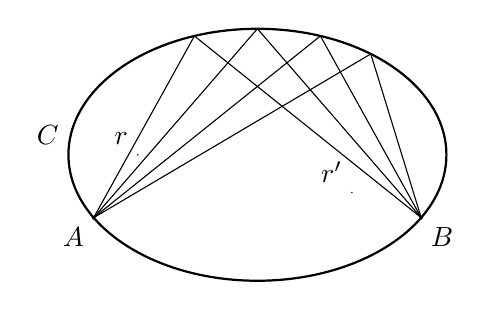
\begin{tikzpicture}[scale=0.8] \draw[thick] (0,0) ellipse (3 and 2);
     \coordinate (A) at (-2.6, -{sqrt(4-(-2.6)*(-2.6)*0.444)}) ;
    \coordinate (C) at (-3,0);
    \coordinate (B) at (2.6, -{sqrt(4-(2.6)*(2.6)*0.444)});
    \foreach \c in {-1,0,1,1.8}{
           \draw[shorten >=-0cm, shorten <=-0cm] (A) -- (\c, {sqrt(4-\c*\c*0.444)});
           \draw[shorten >=-0cm, shorten <=-0cm] (B) -- (\c, {sqrt(4-\c*\c*0.444)});}
    \draw (A) circle [radius=0.02] node[below left] {$A$}; 
    \draw (B) circle [radius=0.02] node[below right] {$B$}; 
    \draw (C) circle [radius=0.0001] node[above left] {$C$};  
    \draw (-1.9,0) circle [radius=0.0001] node[above left] {$r$};
    \draw (1.5,-0.6) circle [radius=0.0001] node[above left] {$r'$};
    \end{tikzpicture}\vspace{-20mm}$$  que se comprueba que es una proyectividad.
\end{teo}
\begin{dem} $\Rightarrow)$
    Elegimos como sistema de referencia $\{A,B,C;u\}$ siendo $C=r\cap\sigma(r)=r\cap r'$ de forma que la recta $A+B=\{x_2=0\}$, $r=A+C=\{x_1=0\}$ y $r'=B+C=\{x_o=0\}$, y tenemos que sacar $\sigma:h_A \longrightarrow h_B$. Elegimos $\sigma$ tal que
     $$\bt h_A \rar{\sim} & h_B \\[-5mm] r \arrow[mapsto]{r} & A+B \\[-5mm] A+B \arrow[mapsto]{r} & r' \et $$ por ser proyectividad. As\'i pues $$\mathbb P^1 \simeq h_A \equiv \lambda x_1 + \lambda x_2 = 0 \qquad \mathbb P^1\simeq h_B \equiv \mu_1 x_2 + \mu_2 x_o = 0$$
     de forma que 
     $$\bt (1:0) \rar{\sigma} & (1:0) \\[-5mm] (0:1) \rar & (0:1)\et$$
     entonces eligiendo como coordenadas $\theta =\frac{\lambda_2}{\lambda_1}$ y $\theta'=\frac{\mu_2}{\mu_1}$, $\sigma$ es afinidad y por ser sobre $\mathbb P^1$ es una homograf\'ia, $\theta' = \frac{a\theta + b}{c\theta +d}$ y la matriz de $\sigma \leadsto \left( \begin{smallmatrix}
         \alpha_1 & 0 \\ 0 & \alpha_2
     \end{smallmatrix}\right)$
     de forma que
     $$\theta' = \frac{a\theta + b}{c\theta +d}= \frac{\alpha_1\theta + 0}{0\theta +\alpha_2} = \dfrac{\alpha_1}{\alpha_2} \theta = k\theta$$
     y por tanto
     $$0=x_1+\theta x_2 \equiv (1,\theta)=s\in h_A \longrightarrow \sigma(s)=s' \equiv (1,\theta') = (1,k \theta ) \equiv 0=x_2+k\theta x_o\in h_B$$
     y hagamos la intersecci\'on de estas rectas:
     $$s\cap \sigma(s) = \begin{cases}
         x_1+\theta x_2=0 \Rightarrow \theta = - \dfrac{x_1}{x_2}\\[5mm] x_2+k \theta x_o=0 \Rightarrow x_2-k \dfrac{x_1x_o}{x_2}=0 \iff x_2^2-kx_1x_o=0
     \end{cases}$$
     lo cual es una c\'onica. Es decir, los puntos $(x_o:x_1:x_2)=s\cap \sigma(s)$ con $s\in h_A$ verifican la ecuaci\'on $x^2_2-kx_1x_0=0$, que es una c\'onica, de matriz $\left(\begin{smallmatrix}
         0 & -1 & 0 \\ -1 & 0 & 0 \\ 0 & 0 & 1
     \end{smallmatrix}\right)$ que es no degenerada, por suponer que $\sigma(A+B)\neq A+B$. Comprobemos que $t_A\equiv r$ y $t_B\equiv r'$. Veamos que $t_A$ es la polar en $A$:
     $$\begin{pmatrix}
         0 & -1 & 0 \\ -1 & 0 & 0 \\ 0 & 0 & 1
     \end{pmatrix}\begin{pmatrix}
         1 \\ 0 \\ 0
     \end{pmatrix} = \begin{pmatrix}
         0 \\ -1 \\ 0
     \end{pmatrix}\Rightarrow \text{ polar de } A \equiv  \{x_1 = 0\} = r$$
     Igual para $t_B$. 

     Supongamos ahora que $\sigma(A+B)=A+B$. Podemos pensar en el dual, de forma que $(h_A)^* = r_A \subset (\mathbb P^2)^*$ y $(h_B)^* = r_B \subset (\mathbb P^2)^*$ y $(A+B)^*=r_A\cap r_B=p_{A+B}$, de forma que $\sigma$ es una perspectividad, pues deja un punto invariante $p_{A+B}$, y existe $V \in (\mathbb P^2)^*$, tal que $(V)^* = r_V\subset \mathbb P^2$. Sea pues $s\in h_A$, $p_s\in r_A$, $\sigma(p_s)=(p_s + V) \cap r_B$ (dicho en $(\mathbb P^2)^*$), que es $\sigma(s)=(s\cap r_V) + B$ y por tanto, $s \cap \sigma(s) = s\cap r_V$, luego todos los puntos homol\'ogos est\'an en $r_V$ y a su vez en $A+B$ por lo que la c\'onica es un par de rectas, que es una c\'onica degenerada.

     $\Leftarrow)$ Si la c\'onica es singular, $A+B$ es una de las rectas del lugar geom\'etrico de la c\'onica, y la perspectividad es para cualquier recta que pasa por $A$, cortar con la otra recta y unir con $B$: 
     $$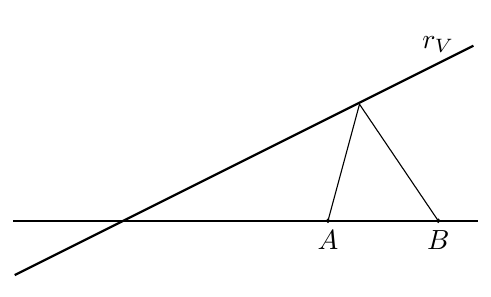
\begin{tikzpicture}[scale=2]
         \draw[shorten >=-0.5cm, shorten <=-0.2cm,thick] (-0.6,0)--(2,0);
         \draw[shorten >=-0.5cm, shorten <=-0.2cm,thick] (-0.6,-0.3)--(2,1) node[above]{$r_V$};
         \coordinate (A) at (1.3,0);\coordinate (B) at (2,0);\coordinate (V) at (1.5,0.74);
         \draw (A) -- (V) -- (B);
         \draw[fill=black] (A) circle [radius=0.01] node[below] {$A$}; 
         \draw[fill=black] (B) circle [radius=0.01] node[below] {$B$}; 
         %\draw[fill=black] (V) circle [radius=0.01] node[above=0.2cm] {$V$};
    \end{tikzpicture}$$
     En el caso en que sea no singular, 
     $$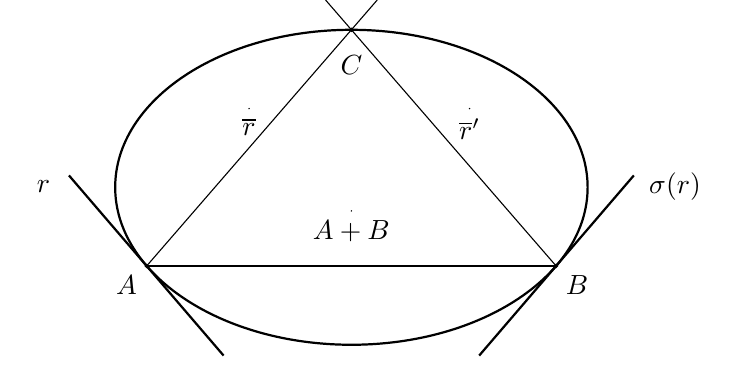
\begin{tikzpicture}[scale=1] \draw[thick] (0,0) ellipse (3 and 2);
    \coordinate (A) at (-2.6, -{sqrt(4-(-2.6)*(-2.6)*0.444)}) ;
    \coordinate (C) at (0, {sqrt(4)});
    \coordinate (B) at (2.6, -{sqrt(4-(2.6)*(2.6)*0.444)});
    \draw (A) circle [radius=0.02] node[below left] {$A$}; 
    \draw (B) circle [radius=0.02] node[below right] {$B$}; 
    \draw (C) circle [radius=0.02] node[below=0.2cm] {$C$};
    \draw (0,-0.3) circle [radius=0.00001] node[below] {$A+B$};
    \draw (-1.3,1) circle [radius=0.00001] node[below] {$\overline{r}$};
    \draw (1.5,1) circle [radius=0.00001] node[below] {$\overline{r}'$};
    \draw[shorten >=-0.5cm, shorten <=-0cm] (A) -- (C);
    \draw[shorten >=-0cm, shorten <=-0.5cm] (C) -- (B);
    \draw[shorten >=-0cm, shorten <=0cm] (B) -- (A);
    \draw[shorten >=-1.5cm, shorten <=-1.5cm,thick] (B) -- (2.61,-{sqrt(4-(2.61)*(2.61)*0.444)}) node[xshift=1.5cm,yshift=1cm] {$\sigma(r)$};    
    \draw[shorten >=-1.5cm, shorten <=-1.5cm,thick] (A) -- (-2.61,-{sqrt(4-(2.61)*(2.61)*0.444)}) node[xshift=-1.3cm,yshift=1cm] {$r$}; 
    \end{tikzpicture}$$
     y construimos una proyectividad 
     $$\bt \overline{\sigma} : h_A \rar & h_B \\[-5mm] A+B \arrow[mapsto]{r} & t_B \\[-5mm] t_A \arrow[mapsto]{r} & A+B \\[-5mm] \overline r \arrow[mapsto]{r}& \overline r' 
     \et$$
     Sea $K$ la c\'onica del lugar geom\'etrico de los puntos de corte de rectas hom\'ologas para $\overline{\sigma}$, de forma que tenemos 3 puntos $A,B,C\in K$, y las tangentes $\overline{\sigma}(t_A)=A+B$ y $\overline{\sigma}(A+B) = t_B$ y $K$ es \'unica, que es la misma de partida, de forma que la aplicaci\'on entre los haces $\sigma$ coincide con la proyectividad $\overline{\sigma}$.
\end{dem}
\begin{defi}
    Sean $A,B,C,D \in K$ una c\'onica, se define la raz\'on doble de $(A,B;C,D)$ como la raz\'on doble de las rectas $(VA,VB;VC,VD)$ ($V\in K$), que no depende del punto $V$ elegido, pues por el rec\'iproco del Teorema de Steiner $\sigma(VA)=V'A, \, \sigma(VB)=V'B, \, \sigma(VC)=V'C, \, \sigma(VD)=V'D$ que es una proyectividad, que mantiene las razones dobles. 
    $$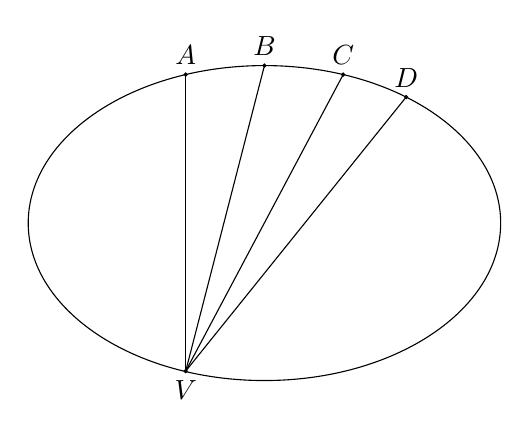
\begin{tikzpicture} \draw (0,0) ellipse (3 and 2);
    \coordinate (V) at (-1,-1.88);
    \foreach \c in {-1,0,1,1.8}{
           \draw[shorten >=-0cm, shorten <=-0cm] (V) -- (\c, {sqrt(4-\c*\c*0.444)});}
    \draw (-1, {sqrt(4-(-1)*(-1)*0.444)}) circle [radius=0.02] node[above] {$A$}; 
    \draw (0, {sqrt(4)}) circle [radius=0.02] node[above] {$B$}; 
    \draw (1, {sqrt(4-(1)*(1)*0.444)}) circle [radius=0.02] node[above] {$C$};
    \draw (1.8, {sqrt(4-(1.8)*(1.8)*0.444)}) circle [radius=0.02] node[above] {$D$}; 
    \draw (V) circle [radius=0.02] node[below] {$V$}; 
    \end{tikzpicture}$$
\end{defi}
\begin{teo}
    Toda c\'onica $C\simeq \mathbb P^1$. Lo que hacemos es identificar $\mathbb P^1\simeq h_V$, de forma que $A \longmapsto V+A$ y $V \longmapsto t_V$, $r\cap C \leftarrow r$. 
\end{teo}